\documentclass{urdpl}

\usepackage[english,polish]{babel}
\usepackage{polski}
\usepackage[utf8]{inputenc}
\usepackage{mathtools}
\usepackage{amsfonts}
\usepackage{amsmath}
\usepackage{amsthm}
\usepackage[hidelinks]{hyperref}
\usepackage{float}
\usepackage{listings}
\usepackage{graphicx}
\usepackage{booktabs}
\usepackage{multirow} 
\usepackage{tabularx} 
\usepackage{amssymb} 
\usepackage{xcolor}
\usepackage{array}
\usepackage{afterpackage}
\usepackage{makecell}
\usepackage[flushleft]{threeparttable}
\usepackage[normalem]{ulem}
\usepackage{lineno}
\usepackage{indentfirst}
\usepackage{titlesec}
\usepackage{siunitx}
\usepackage{courier}





\lstloadlanguages{Java}
\renewcommand{\lstlistlistingname}{Spis listingów}
\renewcommand{\lstlistingname}{Listing}

\lstset{
    literate={ą}{{\k{a}}}1 {ć}{{\'c}}1 {ę}{{\'e}}1 {ó}{{\'o}}1 
             {ń}{{\'n}}1 {ł}{{\l{}}}1 {ś}{{\'s}}1 {ź}{{\'z}}1 
             {ż}{{\.z}}1 {Ą}{{\k{A}}}1 {Ć}{{\'C}}1 {Ę}{{\'E}}1 
             {Ó}{{\'O}}1 {Ń}{{\'N}}1 {Ł}{{\L{}}}1 {Ś}{{\'S}}1 
             {Ź}{{\'Z}}1 {Ż}{{\.Z}}1,
    basicstyle=\footnotesize\ttfamily,
}

\lstdefinestyle{javaStyle}{
    language=Java,
    basicstyle=\ttfamily\footnotesize,
    keywordstyle=\color{blue},
    commentstyle=\color{green!50!black}\itshape,
    stringstyle=\color{red},
    numberstyle=\tiny\color{gray},
    numbers=left,
    numbersep=5pt,                      
    stepnumber=1,
    showspaces=false,                  
    tabsize=2,
    showstringspaces=false,
    breaklines=true,
    breakatwhitespace=false,        
    showtabs=false,                    
    keepspaces=true                 
}


\author{Mikołaj Kopacz}
\shortauthor{M. Kopacz}
\noAlbum{134926}

\titlePL{Projekt i implementacja systemu automatu z napojami z wykorzystaniem języka Java i bazy danych SQLite}
\titleEN{Design and implementation of a beverage vending machine system using Java and SQLite database}

\shorttitlePL{System automatu z napojami w Javie} 
\shorttitleEN{Beverage Vending System in Java}

\thesistype{Praca projektowa}
\thesisDone{Praca wykonana pod kierunkiem}
\supervisor{mgr inż. Ewa Żesławska}

\degreeprogramme{Informatyka}
\date{2025}
\department{Instytut Informatyki}
\faculty{Wydział Nauk Ścisłych i Technicznych}



\makeatletter
\renewcommand{\listoffigures}{%
    \chapter*{\listfigurename}%
    \@starttoc{lof}%
    \thispagestyle{empty}%
}


\renewcommand{\lstlistoflistings}{%
    \chapter*{\lstlistlistingname}%
    \@starttoc{lol}%
    \thispagestyle{empty}%
}
\makeatother


\usepackage[figure,table,lstlisting]{totalcount}
\begin{document}


\titlepages




\tableofcontents
\clearpage


\section{Streszczenie}
\subsection{Streszczenie w języku polskim}
System automatu z napojami to kompleksowe rozwiązanie umożliwiające symulację działania fizycznego automatu vendingowego. Aplikacja została zaimplementowana w języku Java z wykorzystaniem technologii Swing dla interfejsu użytkownika oraz bazy danych SQLite do przechowywania informacji o produktach i transakcjach. W projekcie wykorzystano technologie opisane w \cite{oracle_java} oraz \cite{sqlite_doc}, a także klasę BigDecimal\cite{BigDecimal} dla lepszej jakości obliczeń. System oferuje dwie główne ścieżki interakcji: dla klientów (przeglądanie asortymentu, składanie zamówień, płatności) oraz dla administratorów (zarządzanie stanem magazynowym, monitoring transakcji, analiza finansowa).

\subsection{Summary in English}
The beverage vending machine system is a comprehensive solution simulating the operation of a physical vending machine. The application was implemented in Java using Swing for the user interface and SQLite database for storing product and transaction information.The project utilizes technologies described in \cite{oracle_java} and \cite{sqlite_doc}, as well as BigDecimal class\cite{BigDecimal}, for better quality calculations. The system offers two main interaction paths: for customers (browsing products, placing orders, payments) and for administrators (inventory management, transaction monitoring, financial analysis).
\section{Opis założeń projektu}
\subsection{Cel projektu}
Głównym celem projektu było stworzenie wirtualnego automatu z napojami, który:
\begin{itemize}
\item Symuluje rzeczywiste zachowanie automatu vendingowego
\item Umożliwia łatwe zarządzanie produktami przez administratora
\item Zapewnia intuicyjny interfejs dla użytkowników
\item Rejestruje historię transakcji
\item Generuje raporty finansowe
\end{itemize}




\subsection{Wymagania funkcjonalne}
\begin{itemize}
\item Przeglądanie dostępnych produktów z podziałem na kategorie
\item System koszyka zakupowego
\item Obsługa płatności gotówką i kartą
\item Panel administracyjny z autentykacją
\item Zarządzanie stanem magazynowym
\item Generowanie raportów transakcji
\item Kalkulacja zysków 
\end{itemize}


\subsection{Wymagania niefunkcjonalne}
\begin{itemize}
\item Wydajność: czas reakcji < 1s dla podstawowych operacji
\item Bezpieczeństwo: ochrona danych transakcji
\item Kompatybilność: Java 8+, Windows/Linux/MacOS
\item Użyteczność: intuicyjny interfejs graficzny
\item Niezawodność: odporność na błędy użytkownika
\end{itemize}
\section{Opis struktury projektu}
\subsection{Architektura systemu}
System został zbudowany w oparciu o wzorzec MVC (Model-Widok-Kontroler):
\begin{itemize}
\item \textbf{Model}: Baza danych SQLite + klasy dziedziny (Produkt, Transakcja itp.)
\item \textbf{Widok}: Interfejs użytkownika zrealizowany w Swing
\item \textbf{Kontroler}: Logika biznesowa aplikacji
\end{itemize}


\subsection{Diagram klas}
\begin{figure}[H]
\centering
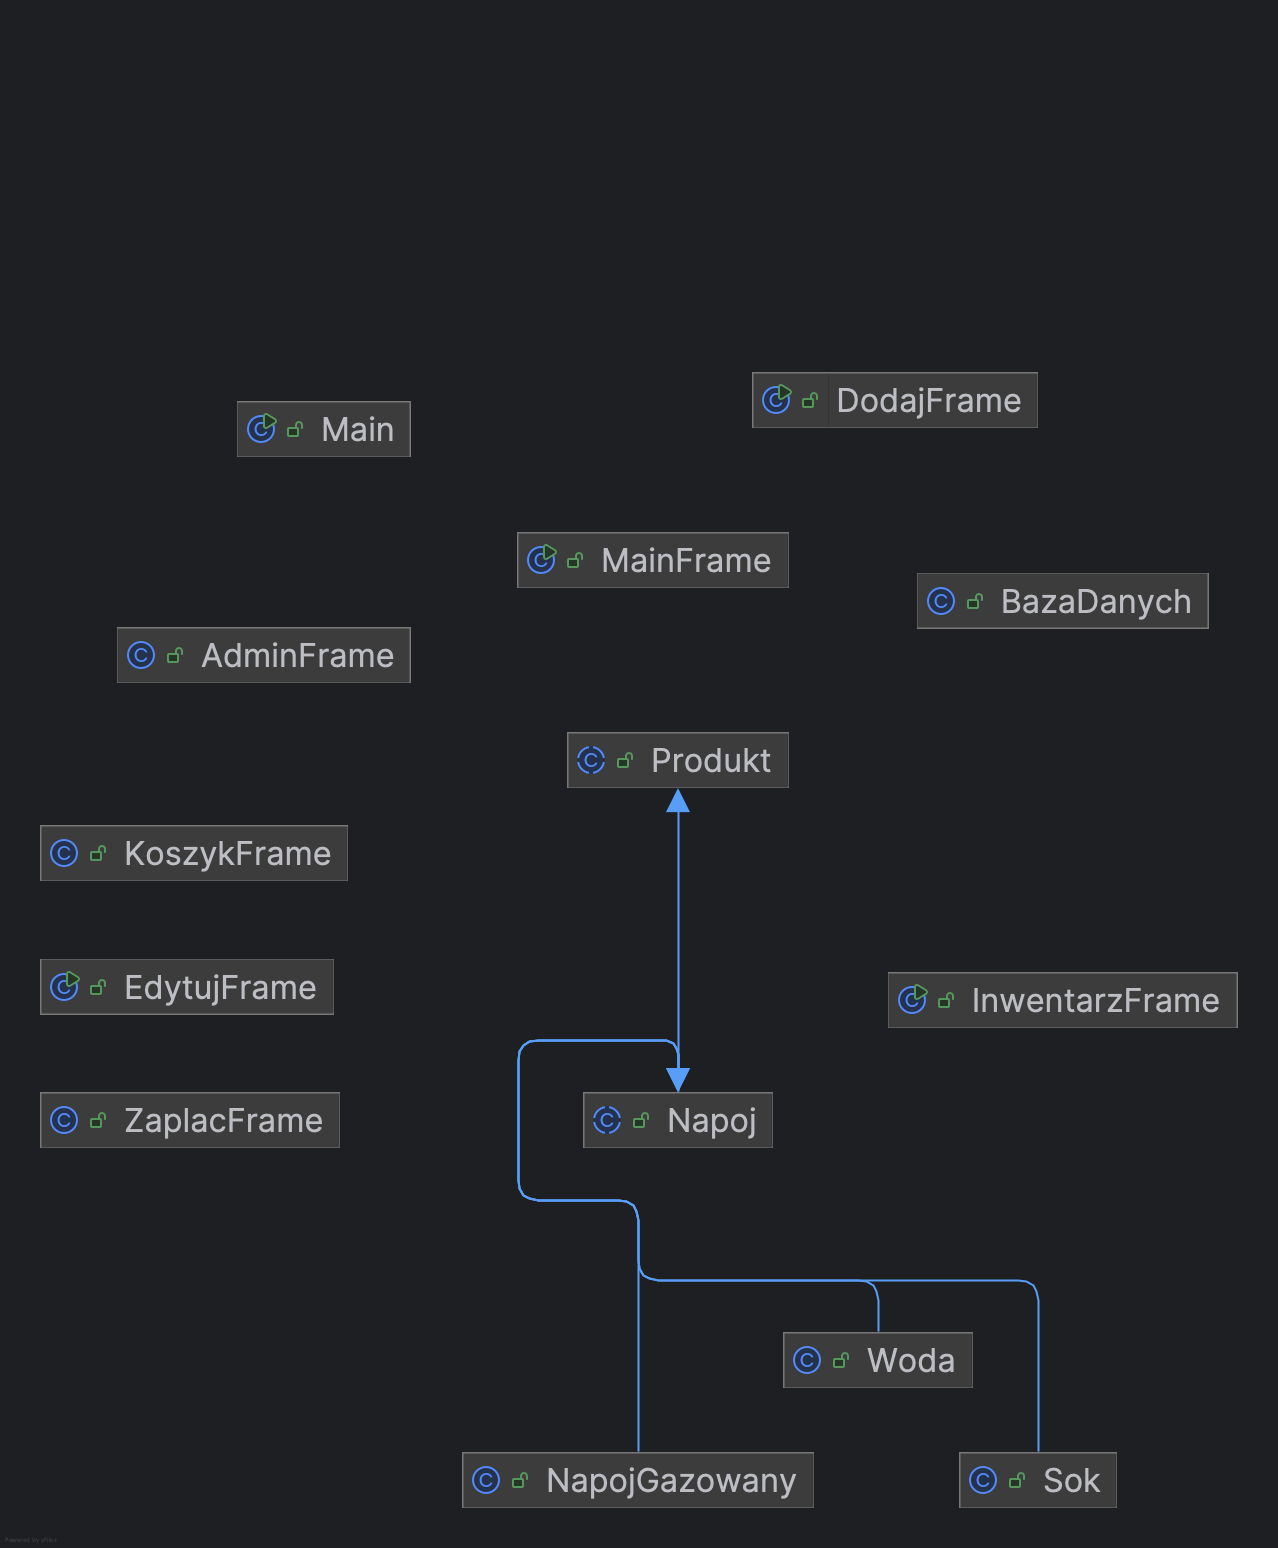
\includegraphics[width=0.9\textwidth]{figures/class_diagram.png}
\caption{Diagram głównych klas systemu}
\label{fig:class_diagram}
\end{figure}

\subsection{Hierarchia dziedziczenia}
System wykorzystuje mechanizm dziedziczenia do modelowania różnych typów produktów. Główna hierarchia klas przedstawia się następująco:

\begin{figure}[H]
\centering
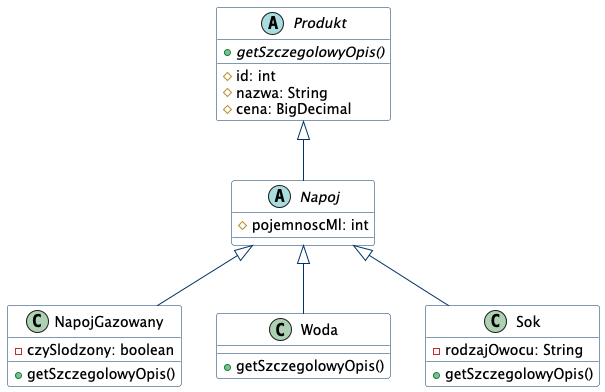
\includegraphics[width=0.7\textwidth]{figures/inheritance_diagram.png}
\caption{Hierarchia dziedziczenia klas produktów}
\label{fig:inheritance_diagram}
\end{figure}

\subsubsection{Klasa bazowa Produkt}
Klasa abstrakcyjna \texttt{Produkt} stanowi podstawę hierarchii:

\begin{lstlisting}[style=javaStyle]
public abstract class Produkt {
    protected int id;
    protected String nazwa;
    protected BigDecimal cena;
    
    public abstract String getSzczegolowyOpis();
}
\end{lstlisting}

\subsubsection{Klasa Napoj}
Klasa \texttt{Napoj} dziedziczy po \texttt{Produkt}, rozszerzając ją o specyficzne dla napojów właściwości:

\begin{lstlisting}[style=javaStyle]
public abstract class Napoj extends Produkt {
    protected int pojemnoscMl;
    
    public Napoj(int id, String nazwa, BigDecimal cena, int pojemnoscMl) {
        super(id, nazwa, cena);
        this.pojemnoscMl = pojemnoscMl;
    }
}
\end{lstlisting}

\subsubsection{Klasy konkretne}
Specyficzne typy napojów dziedziczą po klasie \texttt{Napoj}, implementując własne wersje metody \texttt{getSzczegolowyOpis()}:

\begin{itemize}
\item \texttt{NapojGazowany} - dodaje informację o słodzeniu
\begin{lstlisting}[style=javaStyle, firstnumber=1]
public class NapojGazowany extends Napoj {
    private boolean czySlodzony;
    
    @Override
    public String getSzczegolowyOpis() {
        return String.format("Napój gazowany: %s\nPojemność: %d ml\n(%s)",
            nazwa, pojemnoscMl, czySlodzony ? "słodzony" : "bez cukru");
    }
}
\end{lstlisting}

\item \texttt{Sok} - dodaje informację o rodzaju owocu
\item \texttt{Woda} - podstawowa implementacja dla wody
\end{itemize}

\subsubsection{Zalety zastosowanego podejścia}
\begin{itemize}
\item \textbf{Reużywalność kodu}: Wspólne właściwości są zdefiniowane w klasach nadrzędnych
\item \textbf{Polimorfizm}: Możliwość traktowania różnych typów produktów jednolicie
\item \textbf{Rozszerzalność}: Łatwe dodawanie nowych typów produktów
\end{itemize}

Przykład wykorzystania polimorfizmu w klasie \texttt{BazaDanych}:

\begin{lstlisting}[style=javaStyle]
public static List<Produkt> pobierzWszystkieProdukty() {
    List<Produkt> produkty = new ArrayList<>();
    // ...
    switch (typProduktu) {
        case "GAZOWANY":
            produkty.add(new NapojGazowany(...));
            break;
        case "SOK":
            produkty.add(new Sok(...));
            break;
        // ...
    }
    return produkty;
}
\end{lstlisting}


Kluczowe klasy systemu:
\begin{itemize}
\item \textbf{MainFrame}: Główne okno aplikacji
\item \textbf{Produkt}: Klasa abstrakcyjna reprezentująca produkt
\item \textbf{Napoj}, \textbf{NapojGazowany}, \textbf{Woda}, \textbf{Sok}: Hierarchia klas produktów
\item \textbf{KoszykFrame}: Obsługa koszyka zakupowego
\item \textbf{ZaplacFrame}: Logika płatności
\item \textbf{BazaDanych}: Warstwa dostępu do danych
\end{itemize}



\subsection{Baza danych}
System wykorzystuje lekką bazę danych SQLite z następującymi tabelami:
\begin{itemize}
\item \textbf{produkty} (id, nazwa, cena, typ, ilość)
\item \textbf{detale\_napoje} (id\_produktu, pojemność\_ml)
\item \textbf{transakcje} (id, data, produkty, kwota, metoda\_płatności)
\end{itemize}

\begin{figure}[H]
\centering
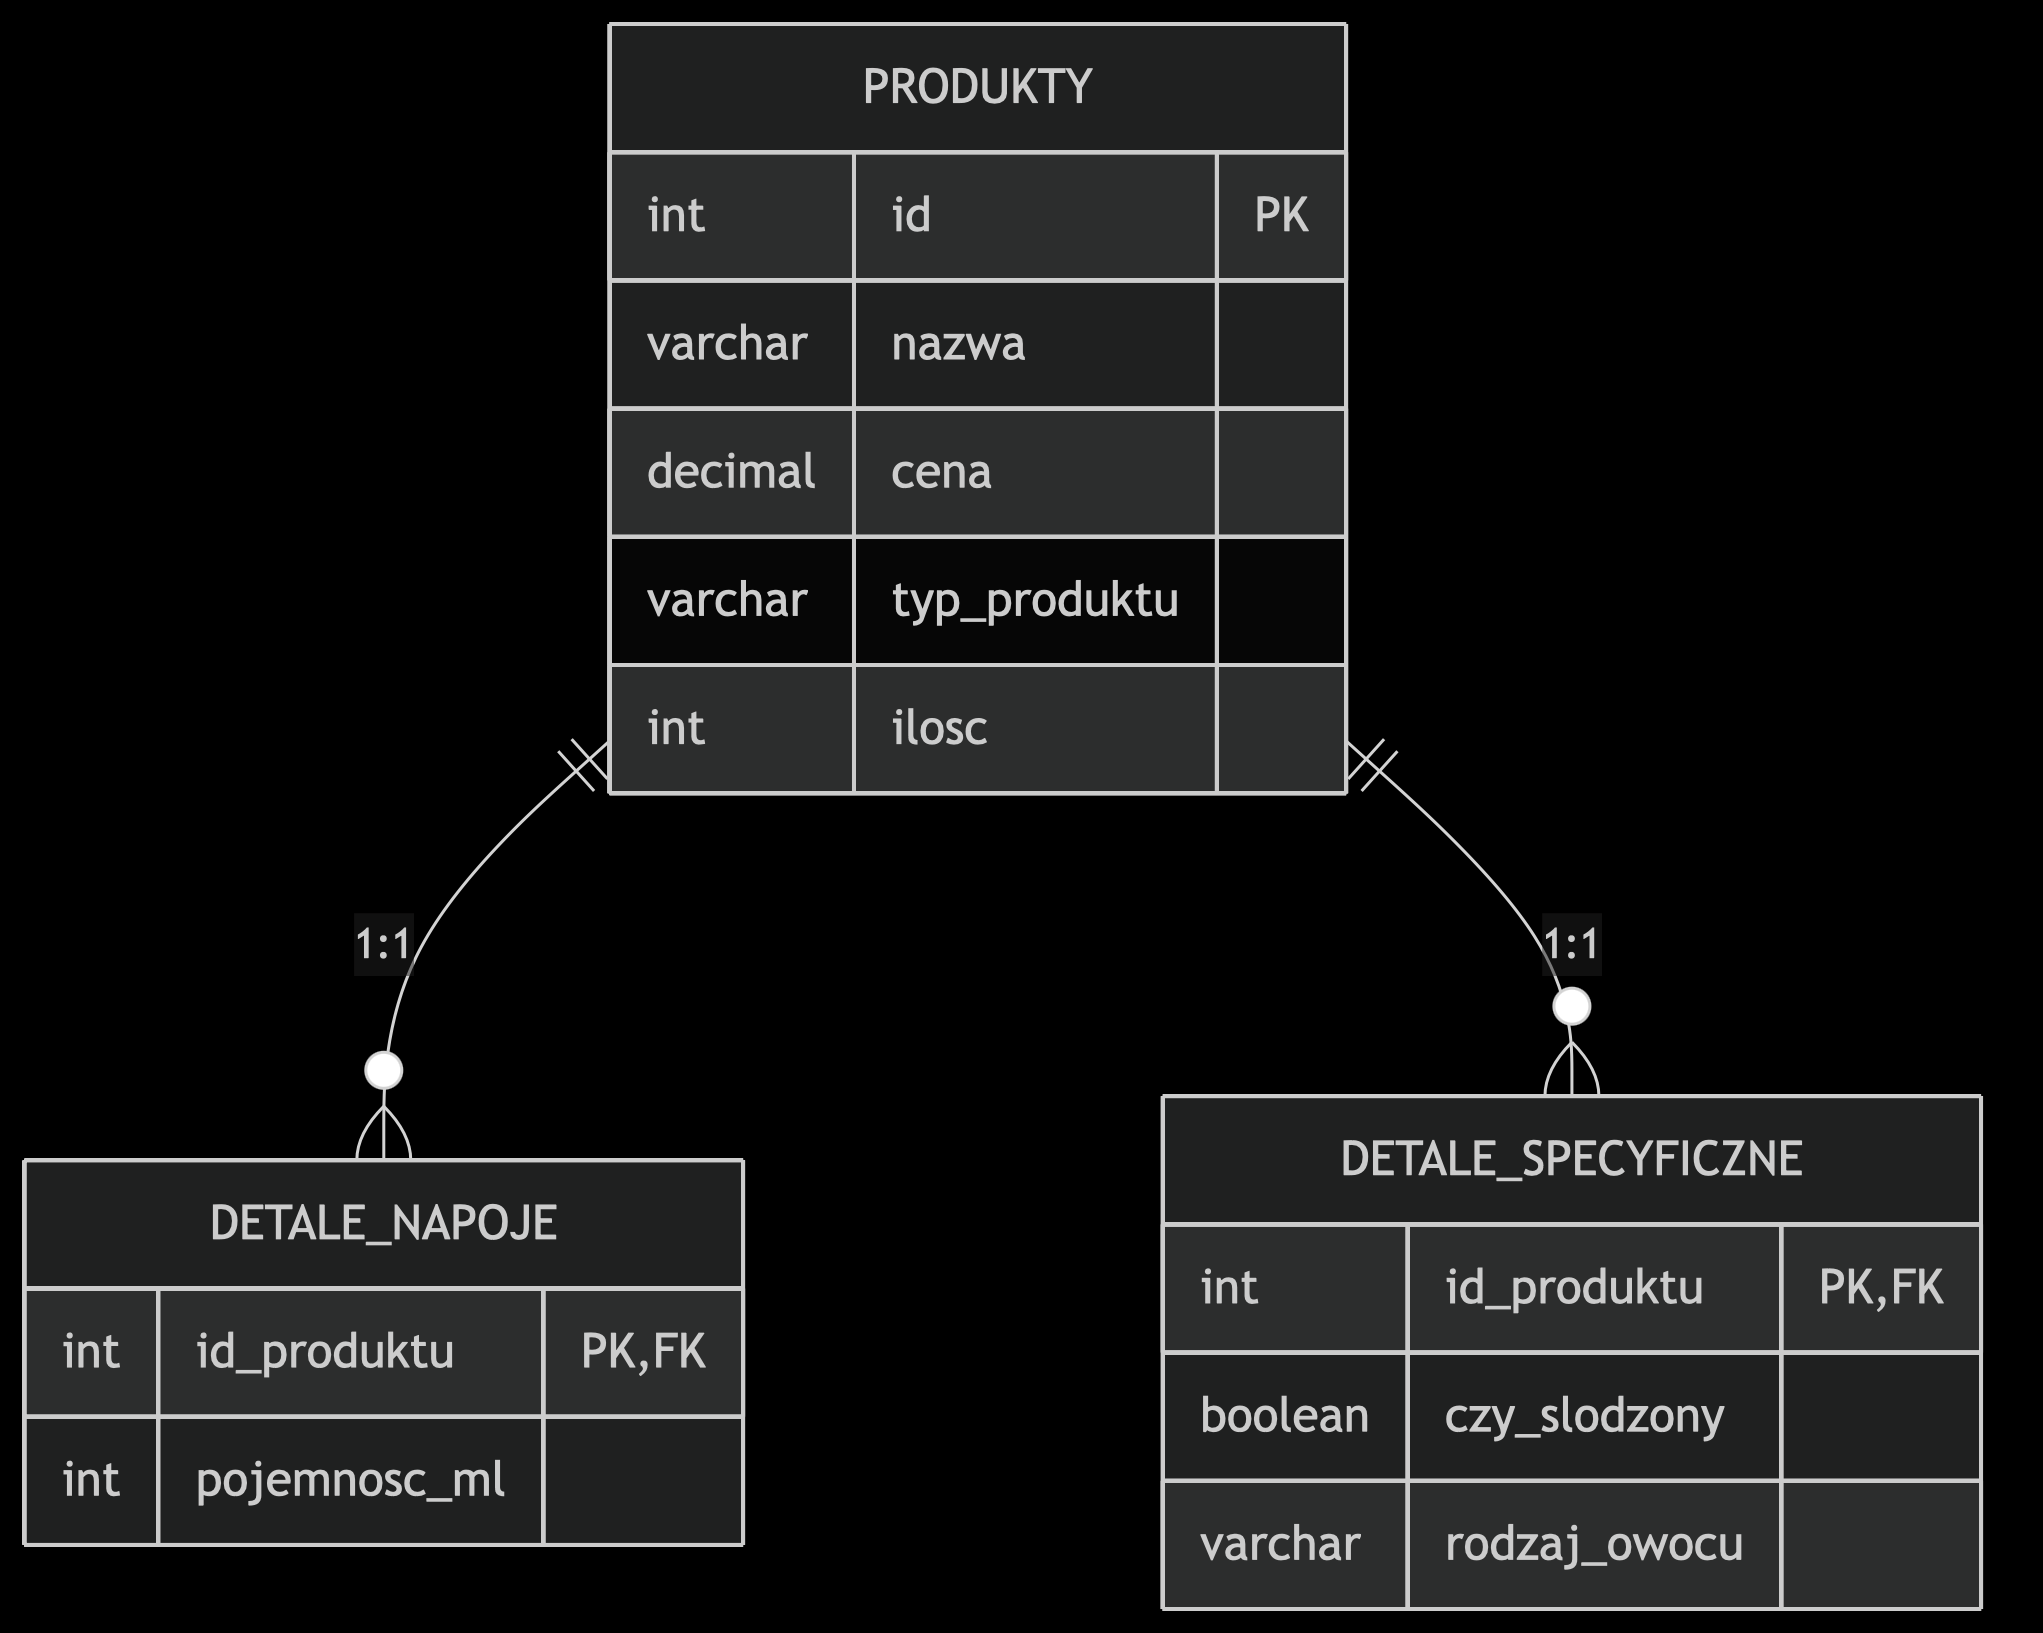
\includegraphics[width=0.8\textwidth]{figures/erd_diagram.png}
\caption{Diagram ERD bazy danych}
\label{fig:erd_diagram}
\end{figure}
\section{Harmonogram realizacji projektu}
Projekt był realizowany według następującego harmonogramu:

\begin{figure}[H]
\centering
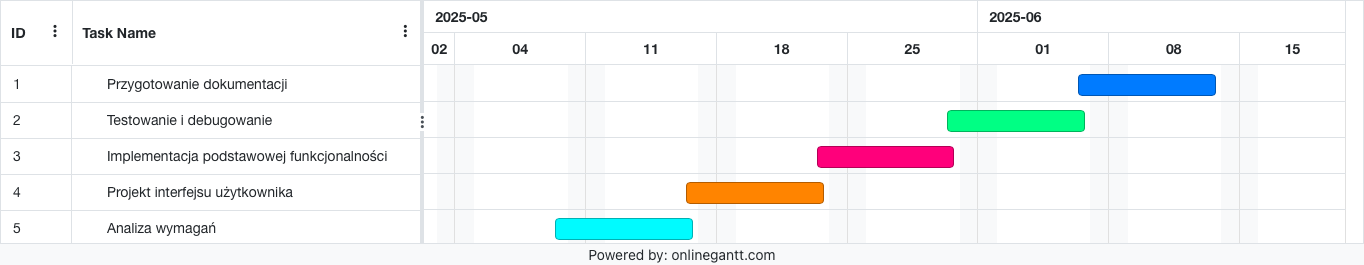
\includegraphics[width=\textwidth]{figures/gantt_chart.png}
\caption{Diagram Ganta realizacji projektu}
\label{fig:gantt}
\end{figure}

Główne etapy realizacji:
\begin{itemize}
\item Analiza wymagań (1 tydzień)
\item Projekt interfejsu użytkownika (1 tydzień)
\item Implementacja podstawowej funkcjonalności (1 tydzień)
\item Testowanie i debugowanie (1 tydzień)
\item Przygotowanie dokumentacji (1 tydzień)
\end{itemize}



Kod źródłowy projektu jest dostępny w repozytorium GitHub: \url{https://github.com/mikolaj-kopacz/System-Automat-Z-Napojami}
\section{Prezentacja warstwy użytkowej projektu}
\subsection{Interfejs użytkownika}
System oferuje dwa główne interfejsy:
\begin{itemize}
\item Interfejs klienta - do składania zamówień
\item Panel administratora - do zarządzania systemem
\end{itemize}

\begin{figure}[H]
\centering
\begin{subfigure}{0.45\textwidth}
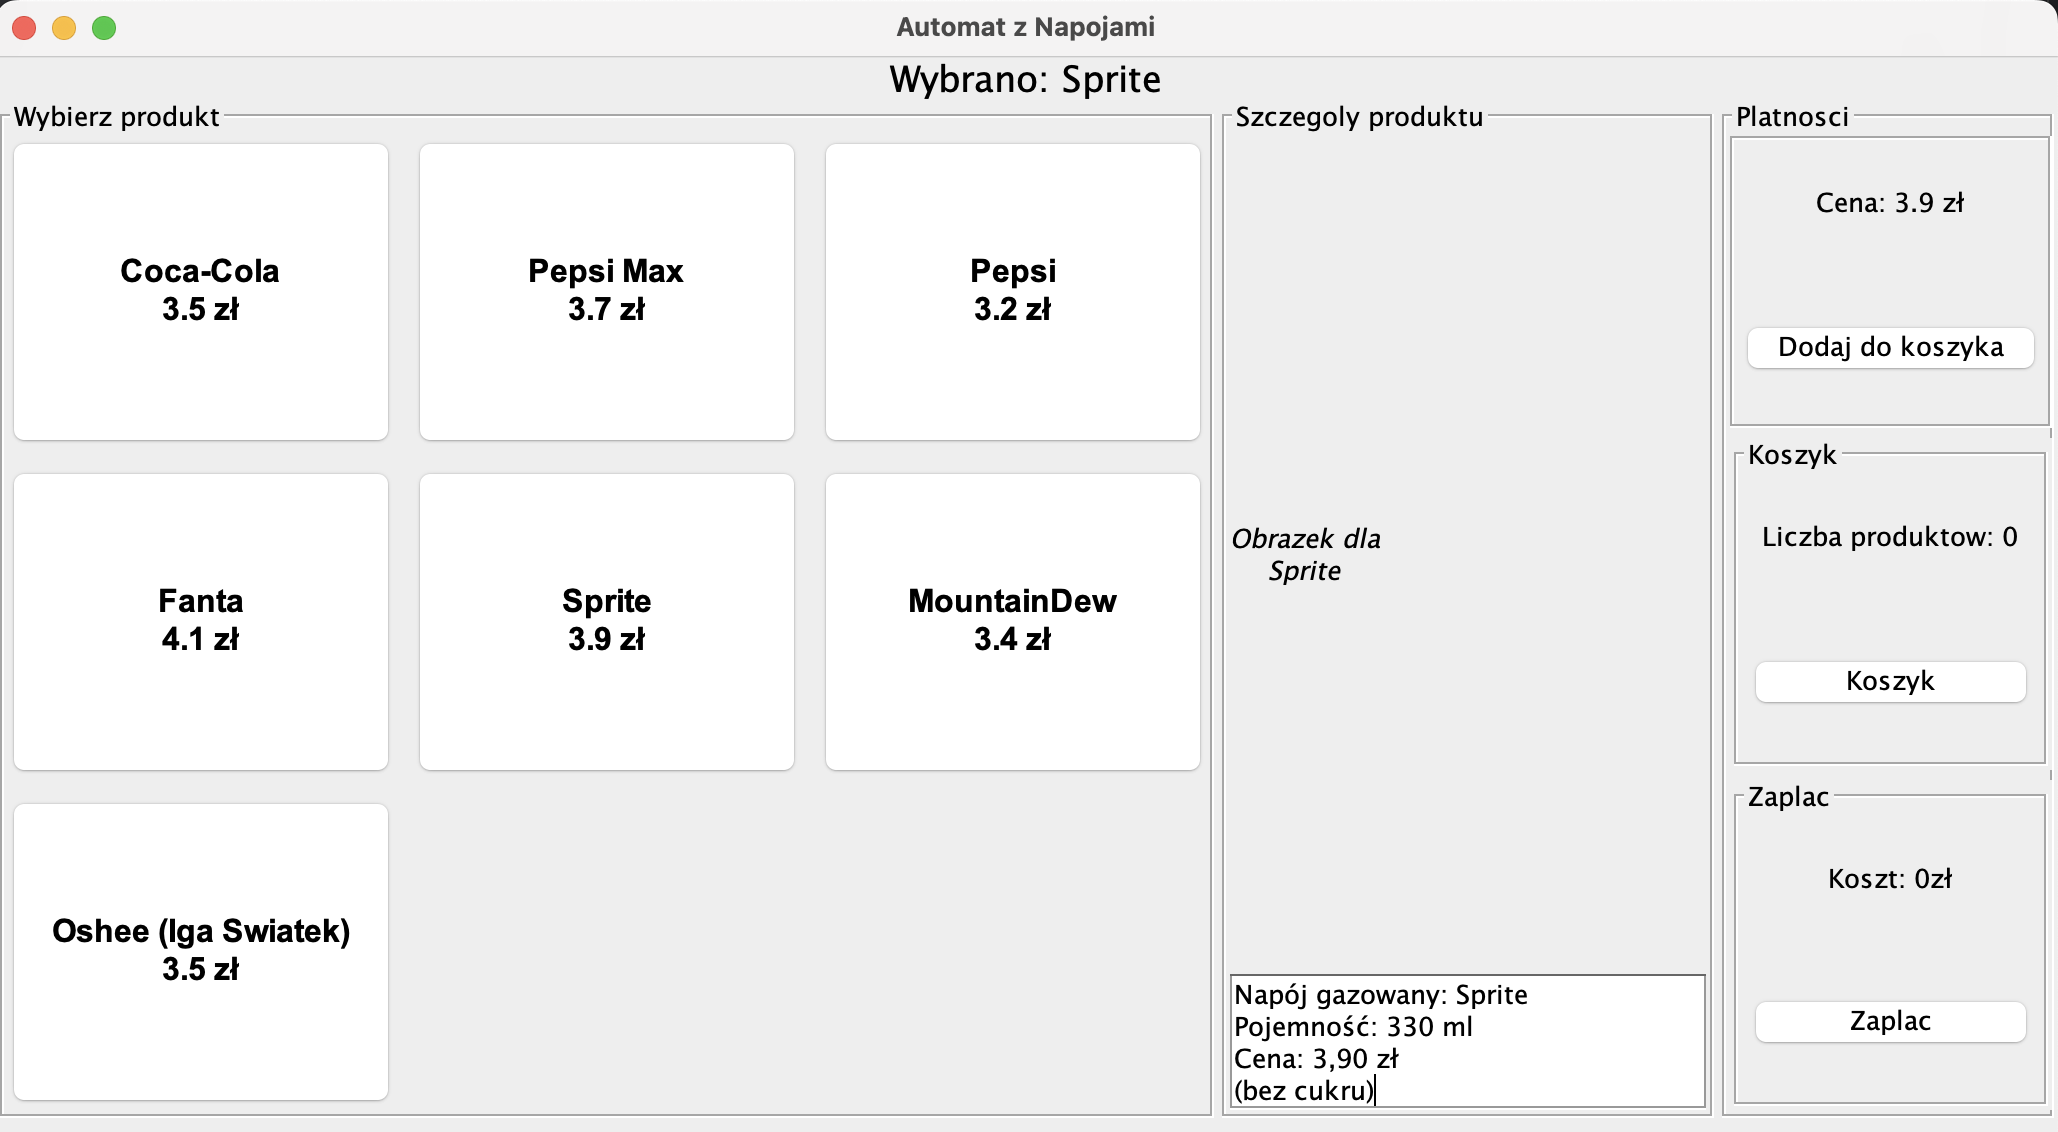
\includegraphics[width=\textwidth]{figures/main_screen.png}
\caption{Ekran główny - wybór produktów}
\label{fig:main_screen}
\end{subfigure}
\begin{subfigure}{0.45\textwidth}
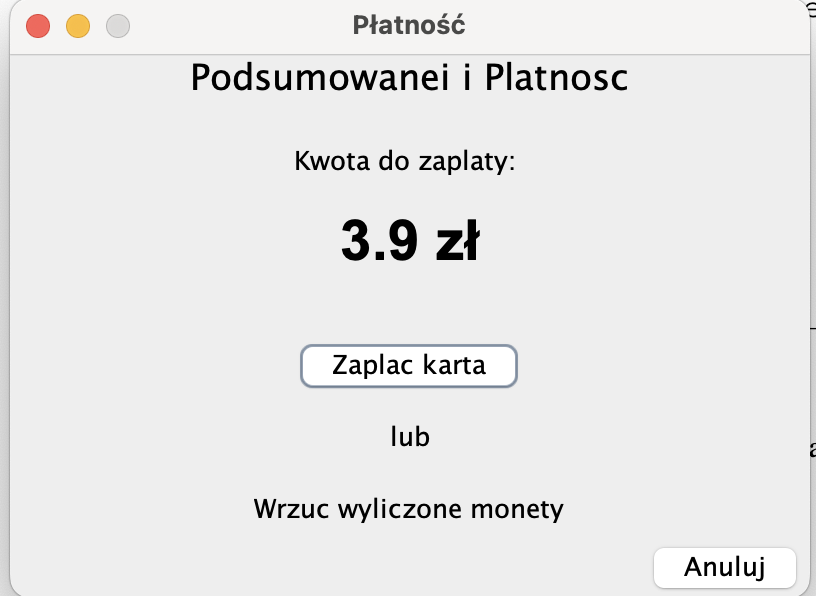
\includegraphics[width=\textwidth]{figures/payment_screen.png}
\caption{Ekran płatności}
\label{fig:payment_screen}
\end{subfigure}
\caption{Podstawowe ekrany systemu}
\end{figure}


\subsection{Przepływ użytkownika}
Typowy scenariusz użycia:
\begin{enumerate}
\item Użytkownik przegląda dostępne produkty
\item Wybiera produkty i dodaje je do koszyka
\item Przechodzi do podsumowania zamówienia
\item Wybiera metodę płatności (gotówka/karta)
\item Otrzymuje potwierdzenie transakcji
\end{enumerate}

\subsection{Panel administratora}
\begin{figure}[H]
\centering
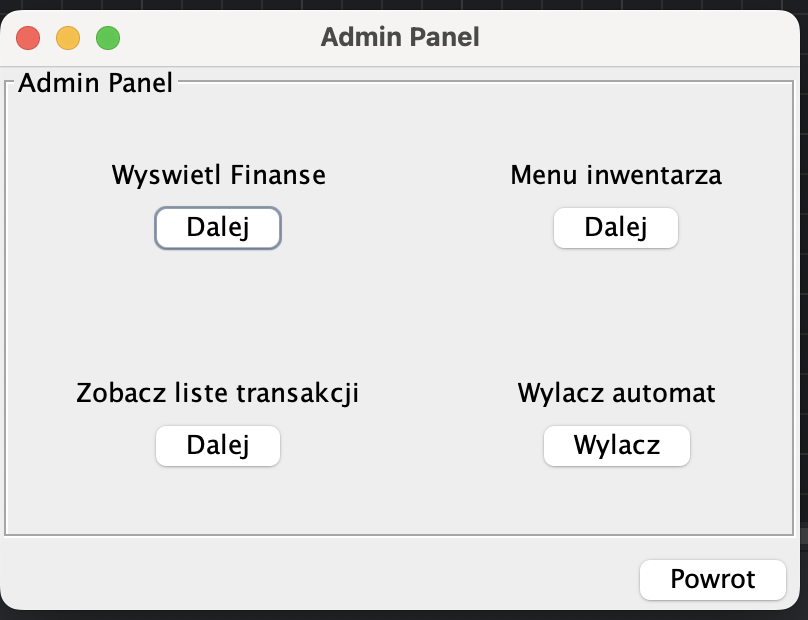
\includegraphics[width=0.7\textwidth]{figures/admin_panel.png}
\caption{Panel administracyjny systemu}
\label{fig:admin_panel}
\end{figure}

Funkcjonalności panelu admina:
\begin{itemize}
\item Zarządzanie produktami (dodawanie, edycja, usuwanie)
\item Przegląd historii transakcji
\item Generowanie raportów finansowych
\item Zarządzanie stanem magazynowym
\end{itemize}
\section{Testowanie systemu}
\subsection{Strategia testowania}
System został przetestowany na trzech poziomach:
\begin{itemize}
\item Testy jednostkowe (JUnit) - poszczególne metody
\item Testy integracyjne - współdziałanie komponentów
\item Testy systemowe - cała aplikacja
\end{itemize}

\subsection{Przykładowe scenariusze testowe}
\begin{table}[H]
\centering
\caption{Przykładowe przypadki testowe}
\begin{tabular}{|l|l|l|}
\hline
\textbf{Scenariusz} & \textbf{Oczekiwany wynik} & \textbf{Status} \\ \hline
Dodanie produktu do koszyka & Koszyk zawiera 1 produkt & PASS \\ \hline
Płatność niewystarczającą kwotą & Komunikat o błędzie & PASS \\ \hline
Logowanie admina poprawnymi danymi & Dostęp do panelu & PASS \\ \hline
\end{tabular}
\end{table}

\subsection{Wyniki testów wydajnościowych}
\begin{itemize}
\item Średni czas ładowania ekranu: 0.3s
\item Maksymalna liczba równoległych transakcji: 15
\item Średni czas przetwarzania płatności: 0.5s
\end{itemize}
\section{Podsumowanie}
\subsection{Osiągnięte cele}
Projekt został zrealizowany zgodnie z założeniami. Wszystkie wymagania funkcjonalne i niefunkcjonalne zostały spełnione. System działa stabilnie i oferuje wszystkie zaplanowane funkcje.


\subsection{Problemy napotkane podczas realizacji}
\begin{itemize}
\item Problemy z synchronizacją dostępu do bazy danych
\item Wyzwania związane z responsywnością interfejsu
\item Optymalizacja wydajności przy dużych zbiorach transakcji
\end{itemize}

\subsection{Kierunki rozwoju}
Możliwe rozszerzenia systemu:
\begin{itemize}
\item Integracja z systemami płatności online
\item Aplikacja mobilna dla administratorów
\item Zaawansowane raporty i analizy sprzedaży
\item Wsparcie dla większej liczby typów produktów
\end{itemize}



\subsection{Wnioski}
Projekt udowodnił, że Java w połączeniu z SQLite stanowią skuteczne narzędzie do budowy systemów vendingowych. Wykonana implementacja może stanowić podstawę dla bardziej zaawansowanych rozwiązań w tej dziedzinie.



\clearpage
\phantomsection
\addcontentsline{toc}{section}{\textbf{Bibliografia}}
\bibliographystyle{plain}
\bibliography{bibliografia.bib}


\clearpage
\phantomsection
\addcontentsline{toc}{section}{\textbf{Spis rysunków}}
\listoffigures


\clearpage
\phantomsection
\addcontentsline{toc}{section}{\textbf{Spis listingów}}
\lstlistoflistings



\clearpage
\phantomsection
\chapter*{}
\label{cha:statement-A}
\makeatletter
\addcontentsline{toc}{section}{\textbf{Oświadczenie studenta o samodzielności pracy}}

\noindent
\begin{flushright}
    \begin{minipage}[!h]{10cm}
        Załącznik nr 2 do Zarządzenia nr 228/2021 Rektora Uniwersytetu Rzeszowskiego z dnia 1 grudnia 2021 roku w sprawie ustalenia procedury antyplagiatowej w Uniwersytecie Rzeszowskim
    \end{minipage}
\end{flushright}

\begin{center}
    \vspace*{10mm}
    \noindent  {\textbf{OŚWIADCZENIE STUDENTA O SAMODZIELNOŚCI PRACY} }
    \vspace*{10mm}
\end{center}

\noindent
\dotuline{\hspace{1.3cm}\@author\hspace{1.3cm}}\\ % Linia pozioma
{\small Imię (imiona) i nazwisko studenta }\\

\noindent \@faculty\\

\noindent \dotuline{\hspace{1.4cm}\@degreeprogramme \hspace{1.4cm}}\\
{\small Nazwa kierunku} \\

\noindent \dotuline{\hspace{1.8cm}\@noAlbum\hspace{1.9cm}}\\
{\small Numer albumu}

\begin{enumerate}
    \item Oświadczam, że moja praca projektowa pt.: \@titlePL
          \begin{enumerate}[label=\arabic*)]
              \item została przygotowana przeze mnie samodzielnie*,
              \item nie narusza praw autorskich w rozumieniu ustawy z dnia 4 lutego 1994 roku o prawie autorskim i prawach pokrewnych (t.j. Dz.U. z 2021 r., poz. 1062) oraz dóbr osobistych chronionych prawem cywilnym,
              \item nie zawiera danych i informacji, które uzyskałem/am w sposób niedozwolony,
              \item nie była podstawą otrzymania oceny z innego przedmiotu na uczelni wyższej ani mnie, ani innej osobie.
          \end{enumerate}
    \item Jednocześnie wyrażam zgodę/nie wyrażam zgody** na udostępnienie mojej pracy projektowej do celów naukowo--badawczych z poszanowaniem przepisów ustawy o prawie autorskim i prawach pokrewnych.
\end{enumerate}


\vspace*{10mm}

\noindent
\underline{\hspace{6cm}} \hfill \underline{\hspace{6cm}} \\ % Puste miejsce na miejscowość, data oraz podpis
\hspace*{13mm}(miejscowość, data)  \hspace*{63mm}(czytelny podpis studenta)
\vspace*{10mm}

\vfill
\noindent
* Uwzględniając merytoryczny wkład prowadzącego przedmiot \\
** -- niepotrzebne skreślić


\end{document}